\documentclass[14pt,a4paper,article]{ncc}
\usepackage[a4paper, mag=1000, left=2.5cm, right=1cm, top=2cm, bottom=2cm, headsep=0.7cm, footskip=1cm]{geometry}
\usepackage[utf8]{inputenc}
\usepackage[T2A]{fontenc}
\usepackage[english,russian]{babel}
\usepackage{indentfirst}
%\usepackage[dvipsnames]{xcolor}
\usepackage{amsfonts} 
\usepackage{amssymb} 
\usepackage{amsmath, etoolbox}
\usepackage{graphicx}
\usepackage{float}
\graphicspath{{../figure/}}
\DeclareGraphicsExtensions{.png,.jpg, .jpeg}

%\bibliographystyle{gost-numeric.bbx}
\usepackage{csquotes}
\usepackage[backend=biber]{biblatex}
\addbibresource{literature.bib}

\usepackage{fancyhdr}
\pagestyle{fancy}
\fancyhead[LE,RO]{\thepage}
\fancyfoot{} 

\usepackage{listings}

\patchcmd\subequations
{\theparentequation\alph{equation}}
{\subequationsformat}
{}{}

\newcommand{\subequationsformat}{\theparentequation.\arabic{equation}}

\numberwithin{equation}{subsection}


\usepackage[colorlinks]{hyperref}
\hypersetup{linkcolor=black}

\begin{document}

% Title page 
\begin{titlepage}
    \begin{center}
        \textsc{
            Санкт-Петербургский политехнический университет имени Петра Великого \\[5mm]
            Институт прикладной математики и механики\\[2mm]
            Кафедра прикладной математики
        }   
        \vfill
        \textbf{\large
            Интервальный анализ\\
            Отчёт по курсовой работе \\[3mm]
        }                
    \end{center}

    \vfill
    \hfill
    \begin{minipage}{0.5\textwidth}
        Выполнил: \\[2mm]   
		Студент: Дамаскинский Константин \\
		Группа: 3630102/70201\\
    \end{minipage}

	\hfill
	\begin{minipage}{0.5\textwidth}
		Принял: \\[2mm]
		к. ф.-м. н., доцент \\   
		Баженов Александр Николаевич
	\end{minipage}

    \vfill
    \begin{center}
        \theyear\ г.
    \end{center}
\end{titlepage}

\tableofcontents
%\listoffigures
%\listoftables
\newpage

\section{Постановка задачи}
\subsection{Задача 1}
Дана матрица 
\begin{equation}
A = 
\begin{pmatrix}
1 & 1\\
1.1 & 1
\end{pmatrix}
\end{equation}

Пусть теперь все элементы матрицы $a_{ij}$ имеют радиус $\varepsilon$:
\begin{equation}
rad \mathbf{a}_{ij} = \varepsilon
\end{equation}

Тогда
\begin{equation}\label{task1}
\mathbf{A} = 
\begin{pmatrix}
[1 - \varepsilon, 1 + \varepsilon] &  [1 - \varepsilon, 1 + \varepsilon] \\
[1.1 - \varepsilon, 1.1 + \varepsilon] & [1 - \varepsilon, 1 + \varepsilon]
\end{pmatrix}
\end{equation}

Требует определить, при каком радиусе $\varepsilon$ матрица \eqref{task1} содержит особенные матрицы.

\subsection{Задача 2}
Дана матрица
\begin{equation}
A = 
\begin{pmatrix}\label{task2}
1 & [0, \varepsilon] & \dots & [0, \varepsilon] \\
[0, \varepsilon] & 1 & \dots & [0, \varepsilon] \\
\vdots & \vdots & \vdots & \vdots \\
[0, \varepsilon] & [0, \varepsilon] & \dots & 1
\end{pmatrix}
\end{equation}

Требует определить, при каком радиусе $\varepsilon$ матрица \eqref{task2} содержит особенные матрицы.

\section{Теория}
\begin{definition}
	Интервальная матрица $\mathbf{A} \in \mathbb{IR}^{n \times n}$ называется \textbf{неособенной}, 
	если неособенны все точечные матрицы $A \in \mathbf{A}$. 
\end{definition}

\begin{definition}
	Если же все точечные матрицы являются особенными, то  $\mathbf{A}$ называется \textbf{особенной}.
\end{definition}

\begin{theorem}
	\textbf{Критерий Баумана} \cite{bazhenov}. Интервальная матрица неособенна тогда и только тогда, когда определители всех её крайних матриц имеют одинаковый знак.
\end{theorem}

%\begin{definition}
%	Говорят, что интервальная матрица имеет \textbf{диагональное преобладание}, если все точечные матрицы, содержащиеся в ней, имеют диагональное преобладание.
%\end{definition}

\begin{theorem}
	\textbf{Признак Бекка} \cite{bazhenov}. Пусть $mid \mathbf{A}$ неособенна ($\mathbf{A} \in \mathbb{IR}^{n \times n}$) и
	$$\rho(\mid (mid \mathbf{A})^{-1} \mid \cdot rad \mathbf{A}) < 1$$
	Тогда $\mathbf{A}$ неособенна.
\end{theorem}


\section{Реализация}

Лабораторная работа выполнена с помощью математического пакета Octave. Операционная система Ubuntu 20.04.

Ссылка на исходный код лабораторной работы и отчёта находится в разделе \hyperref[app]{``Приложения''}.

\section{Результаты}
\subsection{Задача 1}

Субдифференциальный метод Ньютона вернул следующий результат:
\begin{equation}
\mathbf{x} = 
\begin{pmatrix}
1.000 \\
[1.444, 0.636] \\
[0.667, 1.273]
\end{pmatrix}
\end{equation}

Решение производилось с точностью до третьего знака. Невязка решения равна нулю (найденное решение является точным).

\begin{remark}
	Подразумевается ненулевая невязка при подстановке решения вплоть до последнего полученного знака. Однако предъявляется решение именно вплоть до третьего знака, поскольку запрос в методе был именно таковым. Однако, как мы знаем из теоретического раздела, данный метод отыскивает точное решение полиэдральных функций, поэтому полученный результат является отнюдь не удивительным, а закономерным.
\end{remark}

\subsection{Задача 2}

В качестве начального вектора был взят вектор, приложенный в письме (см. \ref{app}).

Сопутствующие задачи с квадратными матрицами были решены с помощью метода, использующего знаково-блочные матрицы. В результате был получен следующий вектор:
\begin{equation}
\mathbf{x}=
\begin{pmatrix}
[0.558, 0.442] \\
[0.697, 0.802] \\
[1.104, 0.895] \\
[0.960, 1.039] \\
[0.751, 0.748] \\
[0.282, 0.717] \\
[0.374, 0.125] \\
[0.523, 0.476] \\
[0.692, 0.807] \\
[0.695, 0.804] \\
[0.469, 0.530] \\
[0.267, 0.232] \\
[0.077, -0.077] \\
[0.321, 0.178] \\
[0.752, 0.247] \\
[0.539, 0.460] \\
[0.408, 0.091] \\
[0.155, -0.155] \\
[2.194, -2.194] \\
[0.389, 0.110] \\
[0.880, 0.119] \\
[0.493, 0.506] \\
[0.673, -0.173] \\
[0.269, -0.269] \\
[0.282, 0.217] \\
[0.629, 0.370] \\
[0.816, 0.683] \\
[0.745, 0.754] \\
[0.390, 0.609] \\
[0.078, 0.421] \\
[0.527, 0.472] \\
[1.382, 0.117] \\
[1.149, 0.850] \\
[1.113, 0.886] \\
[0.795, 0.704] \\
[0.280, 0.719]
\end{pmatrix}
\end{equation}

Правый столбец сгенерирован следующим образом: матрица из файла \texttt{matrix\_n\_phi\_1.txt}, помноженная на вектор $x^{(0)}$ (см. \hyperref[app]{``Приложения''}), определяет $\mathrm{mid} \mathbf{b}$. Вектор объинтерваливается по формуле:

\begin{equation}
\mathbf{b}_i = [\mathrm{mid} \mathbf{b}_i - 0.05 \cdot (i \; \mathrm{mod} \; 7 + 1),
\mathrm{mid} \mathbf{b}_i + 0.05 \cdot (i \; \mathrm{mod} \; 7 + 1)]
\end{equation}

Найденное решение удовлетворяет 144 уравнениям из 256.

Начальный вектор $x^{(0)}$ пересекается с итоговым результатом по 17 компонентам из 36.

Произведение матрицы на вектор-решение не может поместиться на одну страницу данного отчёта, поэтому оно представлено в отдельном файле. Ссылку можно найти в \hyperref[app]{приложениях}.

На следующем графике демонстрируется, как соотносятся компоненты найденного решения и оригинального вектора. Абсцисса соответствует номеру компоненты, ордината -- значению.

Также отражена сумма по столбцам с соответствующими номерами. Этот график представлен в логарифмическом виде. Таким образом, отрицательные числа соответствуют суммам, меньшим единицы.

\begin{figure}[H]
	\begin{center}
		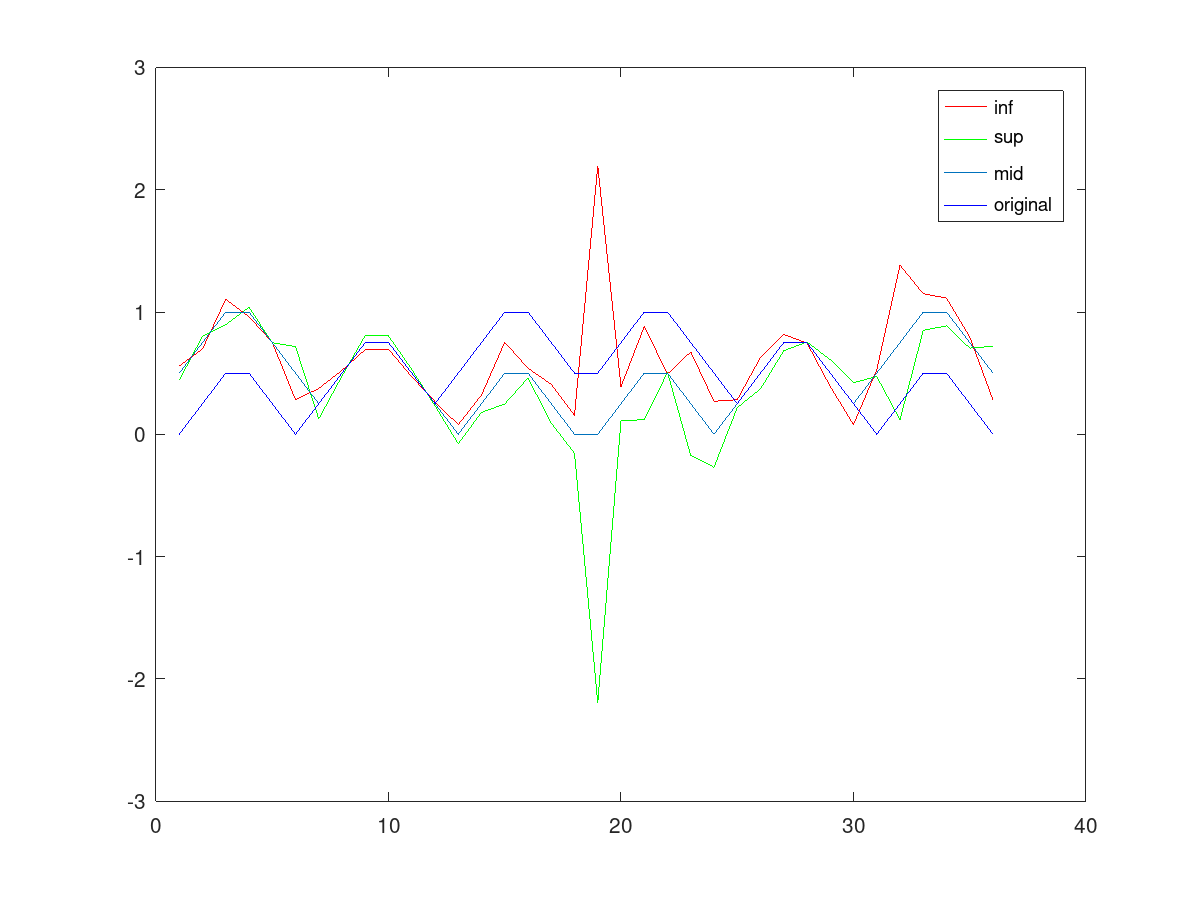
\includegraphics[scale=0.4]{subdiff}
		\caption{$\mathbf{x}, x^{(0)}$, сумма по столбцам}
	\end{center}
\end{figure}

\section{Обсуждение}

В результате проделанной работы была скорректирована правая часть ИСЛАУ с точечной матрицей. Найденное решение в самом деле обеспечило непустоту доускового множества решения, а значит, сработало корректно.

В то же время стоит отметить, что радиус интервала одной из компонент был увеличен очень значительно: с \texttt{0.100} до \texttt{0.476}, что может быть неприемлемо в реальных задачах. Однако, остальные компоненты получили нулевой радиус.

Произведём простейшую оценку корректности полученного результата.
Радиусы правой части составляют:

\begin{equation}
\textrm{rad} \mathbf{b}=
\begin{pmatrix}
0.25 & 0.1 & 0.1
\end{pmatrix}^T
\end{equation}.

Значение максимума распознающего функционала в исходной системе равно приблизительно -0.2. Значит, используя жадный подход, можно расширить все радиусы на 0.2 и гарантированно достичь неотрицательности распознающего функционала и, следовательно, непустоты допускового множества решений. Таким образом, жадный вектор масштабных коэффициентов:

\begin{equation}
\mathbf{w_{greedy}}=
\begin{pmatrix}
\frac{0.25 + 0.2}{0.25} & \frac{0.1 + 0.2}{0.1} & \frac{0.1 + 0.2}{0.1}
\end{pmatrix}^T
=
\begin{pmatrix}
1.8 & 3 & 3
\end{pmatrix}^T
\end{equation}

и его норма: $\|\mathbf{w_{greedy}}\|_1=7.8$

Найденное симплекс-методом решение оптимальнее жадного практически в два раза (в смысле $l_1$-нормы).

\printbibliography
\addcontentsline{toc}{section}{Литература}

\section{Приложения} \label{app}

\begin{enumerate}
	\item Репозиторий с кодом программы и кодом отчёта:
	
	\href{https://github.com/kystyn/interval}{https://github.com/kystyn/interval}
	
	\item Вектор $\mathbf{Ax}$:
	
	\href{https://github.com/kystyn/interval/tree/master/src/subdiff/Ax.txt}{https://github.com/kystyn/interval/tree/master/src/subdiff/Ax.txt}
	
	\item Репозиторий с кодом программы и кодом отчёта:
	
	\href{https://github.com/kystyn/interval}{https://github.com/kystyn/interval}
	
	\item \texttt{subdiff} Сергея Петровича Шарого для SciCodes:
	
	\href{http://www.nsc.ru/interval/Programing/SciCodes/subdiff.sci}{http://www.nsc.ru/interval/Programing/SciCodes/subdiff.sci}

\end{enumerate}

\end{document}
